\Variant{01.12.2024 (3-smena)}
\QQ{1}{$7^{2023}$ sonining onlar xonasidagi raqamni toping.
\Opts{$4$}{$1$}{$3$}{$7$}}
\QQ{2}{Hisoblang:
\[6-\frac{31}{30}-\frac{61}{60}-\frac{101}{100}-\frac{151}{150}-\frac{211}{210}\]
\Opts{$1$}{$\dfrac{15}{13}$}{$\dfrac{142}{185}$}{$\dfrac{13}{14}$}}
\QQ{3}{Agar $A$ va $B$ natural sonlarining köpaytmasi $A\cdot B=3^4\cdot5^2\cdot7^3\cdot11$ ga teng bölsa, EKUB$(A;\,B)$ ning eng katta qiymatini toping.
\Opts{$478$}{$3117$}{$315$}{$319$}}
\QQ{4}{Ikki turli natural sonlarning yiğindisi $36$ va kvadratlari yiğindisi eng kiçik bölsa, ularning köpaytmasini toping.
\Opts{$323$}{$324$}{$325$}{$326$}}
\QQ{5}{Soddalaştiring:
\[\left(\frac{8a^3+b^3}{4a^2-b^2}+b\right):\left(\frac{a^2}{2a-b}\right)\]
\Opts{$2a-b$}{$2a+b$}{$4$}{$1$}}
\QQ{6}{Soddalaştiring:
\[\frac{\left(\sqrt{11}-\sqrt5\right)\left(\sqrt{15}+\sqrt{33}-\sqrt{22}-\sqrt{10}\right)}{\sqrt{108}-\sqrt{72}}\]
\Opts{$1$}{$2$}{$3$}{$4$}}
\QQ{7}{$a$ soni $1,\,4,\,7,\,\dots$ arifmetik progressiyaning biror hadi bölib, quyidagi ifodaning qiymati $2$ ga teng bölsa, $a$ ning qiymatini toping.
\[\frac1{\sqrt4+\sqrt1}+\frac1{\sqrt7+\sqrt4}+\dots+\frac1{\sqrt{a+3}+\sqrt a}=2\]
\Opts{$6$}{$46$}{$9$}{$49$}}
\QQ{8}{Iş haqi dastlab $10\%$ ga, keyin esa $20\%$ ga oşdi. Iş haqi dastlabki holatiga nisbatan neça foizga oşgan?
\Opts{$30$}{$33$}{$32$}{$35$}}
\QQ{9}{$|2x+3|=15$ tenglama ildizlari yiğindisini (agar u bitta bölsa, şu ildizning özini) toping.
\Opts{$-3$}{$-9$}{$-1$}{$6$}}
\QQ{10}{Agar funksiya $f(x)=\dfrac{6x+5}{x+6}$ bölsa, uşbu funksiyaga teskari funksiyani toping.
\Opts{$\dfrac{6x-8}{2-x}$}{$\dfrac{6x-5}{6-x}$}{$\dfrac{x-7}{6-x}$}{$\dfrac{6x+5}{6-x}$}}
\QQ{11}{Agar geometrik progressiya uçun $b_{m+n}=A$ va $b_{m-n}=B$ bölsa, $b_m$ ni toping.
\Opts{$\sqrt{\dfrac AB}$}{$\sqrt{AB}$}{$\sqrt{A-B}$}{$A+B$}}
\QQ{12}{Tekislikda yotmagan $M$ nuqtadan tekislikning $A$ va $B$ nuqtalariga tekislik bilan $30^\circ$ va $60^\circ$ burçak hosil qiluvçi $MA$ va $MB$ oğmalar tuşirildi. Agar $M$ nuqtadan tekislikkaça eng qisqa masofa $2\sqrt3$ bölsa, $A$ va $B$ nuqtalar orasidagi eng qisqa masofani toping.
\Opts{$2\sqrt{10}$}{$6$}{$4$}{$2\sqrt3$}}
\QQ{13}{$ABCDA_1B_1C_1D_1$ kub berilgan bölib, $\overrightarrow{AC}\cdot\overrightarrow{AC_1}=12$ bölsa, kub qirrasi uzunligini toping.
\qfig{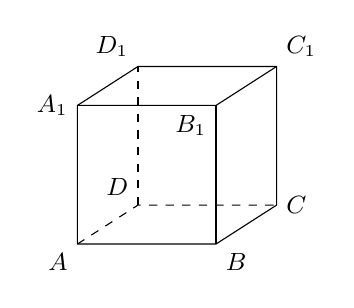
\begin{tikzpicture}[scale=1.1,font=\small]
\coordinate (A) at (0,0); \coordinate (B) at (1.6,0); \coordinate (C) at (2.3,0.45); \coordinate (D) at (0.7,0.45);
\coordinate (A1) at (0,1.6); \coordinate (B1) at (1.6,1.6); \coordinate (C1) at (2.3,2.05); \coordinate (D1) at (0.7,2.05);
\draw (A)--(B)--(C)--(C1)--(D1)--(A1)--cycle; \draw (A1)--(B1)--(C1); \draw (B)--(B1);
\draw[dashed] (A)--(D)--(C); \draw[dashed] (D)--(D1);
\node[below left] at (A) {$A$}; \node[below right] at (B) {$B$}; \node[right] at (C) {$C$}; \node[above left] at (D) {$D$};
\node[left] at (A1) {$A_1$}; \node[below left] at (B1) {$B_1$}; \node[above right] at (C1) {$C_1$}; \node[above left] at (D1) {$D_1$};
\end{tikzpicture}}
\Opts{$\sqrt3$}{$2$}{$\sqrt6$}{$2\sqrt3$}}
\QQ{14}{Agar rasmda muntazam sakkizburçak va muntazam oltiburçak tasvirlangan bölsa, $\alpha$ burçakni toping.
\qfig{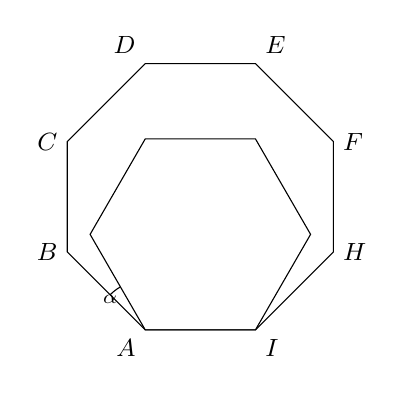
\begin{tikzpicture}[scale=1.4,font=\small]
\coordinate (A) at (0,0); \coordinate (I) at (1,0); \coordinate (H) at (1.707,0.707); \coordinate (F) at (1.707,1.707); \coordinate (E) at (1,2.414); \coordinate (D) at (0,2.414); \coordinate (C) at (-0.707,1.707); \coordinate (B) at (-0.707,0.707);
\draw (A)--(I)--(H)--(F)--(E)--(D)--(C)--(B)--cycle;
\draw (A)--(I)--(1.5,0.866)--(1,1.732)--(0,1.732)--(-0.5,0.866)--cycle;
\draw (A)+(120:0.45) arc (120:135:0.45); \node at (-0.32,0.28) {\scriptsize$\alpha$};
\node[below left] at (A) {$A$}; \node[below right] at (I) {$I$}; \node[right] at (H) {$H$}; \node[right] at (F) {$F$}; \node[above right] at (E) {$E$}; \node[above left] at (D) {$D$}; \node[left] at (C) {$C$}; \node[left] at (B) {$B$};
\end{tikzpicture}}
\Opts{$20^\circ$}{$15^\circ$}{$45^\circ$}{$75^\circ$}}
\QQ{15}{$f(x)=\left|x^2+3x+2\right|$ va $g(x)=-x-1$ funksiyalar bilan çegaralangan soha yuzini toping.
\Opts{$1$}{$\dfrac12$}{$\dfrac32$}{$4$}}
\QQ{16}{Agar $f(x)=\left|\log_{\cos x}\sin x-\ln\pi\right|$ bölsa, $f'\left(\dfrac\pi4\right)$ ni toping.
\Opts{$\log_2e$}{$-4\log_2e$}{$-4\log_4e$}{$4\log_2e$}}
\QQ{17}{$ABC$ töğri burçakli uçburçakka aylana şunday çizilganki, aylana $AB$ katetga urinib şu katet qarşisidagi burçakdan ötadi. Aylana markazi $O$ nuqta $BC$ gipotenuzada joylaşgan, aylana gipotenuzani $E$ nuqtada kesib ötadi. Agar $BE=1$, $OC=4$ va $\angle BCD=\angle ACD$ bölsa, $O$ nuqtadan $DC$ tomongaça bölgan masofani toping.
\qfig{\begin{tikzpicture}[scale=0.55,font=\small]
\coordinate (B) at (0,0); \coordinate (E) at (1,0); \coordinate (O) at (5,0); \coordinate (C) at (9,0); \coordinate (D) at (1.8,2.4); \coordinate (A) at (3.24,4.32);
\draw (O) circle (4); \draw (A)--(B)--(C)--cycle; \draw (D)--(C); \fill (O) circle (3pt);
\draw ($(A)!0.45cm!(B)$)--($(A)!0.45cm!(B)!0.45cm!90:(B)$)--($(A)!0.45cm!(C)$);
\node[above] at (A) {$A$}; \node[left] at (B) {$B$}; \node[right] at (C) {$C$}; \node[above left] at (D) {$D$}; \node[below right] at (E) {$E$}; \node[below] at (O) {$O$};
\node[below] at (0.5,0) {$1$}; \node[below] at (3,0) {$4$}; \node[below] at (7,0) {$4$};
\end{tikzpicture}}
\Opts{$\dfrac{2\sqrt{10}}5$}{$\dfrac{3\sqrt{10}}5$}{$\dfrac{4\sqrt{10}}5$}{$\dfrac{\sqrt{10}}5$}}
\QQ{18}{Agar $ABC$ va $MNC$ uçburçaklar töğri burçakli uçburçaklar va $AB=6$, $MN=3$, $NC=4$ bölsa, $x$ ning qiymatini toping.
\qfig{\begin{tikzpicture}[scale=0.45,font=\small]
\coordinate (B) at (0,0); \coordinate (A) at (0,6); \coordinate (C) at (8,0); \coordinate (N) at (4.8,2.4); \coordinate (M) at (3,0);
\draw (A)--(B)--(C)--cycle; \draw (M)--(N); \draw (0,0.5)--(0.5,0.5)--(0.5,0);
\draw ($(N)!0.4cm!(C)$)--($(N)!0.4cm!(C)!0.4cm!90:(C)$)--($(N)!0.4cm!(M)$);
\node[above] at (A) {$A$}; \node[below left] at (B) {$B$}; \node[below right] at (C) {$C$}; \node[above right] at (N) {$N$}; \node[below] at (M) {$M$};
\node[left] at (0,3) {$6$}; \node[above right] at (2.4,4.2) {$x$}; \node[above right] at (6.4,1.2) {$4$}; \node[left] at (3.9,1.4) {$3$};
\end{tikzpicture}}
\Opts{$5$}{$10$}{$6$}{$9$}}
\QQ{19}{Rombning bir uçi aylana markazida, qolgan uçlari esa aylanada yotadi. Agar şu aylanaga taşqi çizilgan muntazam uçburçak yuzi $48\sqrt3$ bölsa, rombning yuzini toping.
\qfig{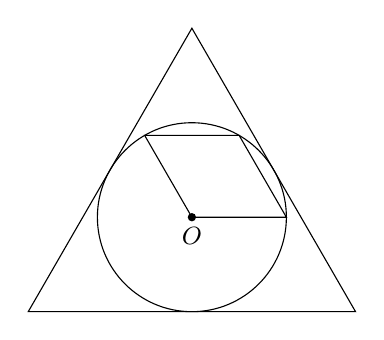
\begin{tikzpicture}[scale=0.3,font=\small]
\draw (0,0) circle (4); \draw (90:8)--(210:8)--(330:8)--cycle;
\draw (0,0)--(0:4)--(60:4)--(120:4)--cycle; \fill (0,0) circle (5pt); \node[below] at (0,0) {$O$};
\end{tikzpicture}}
\Opts{$8$}{$16$}{$4\sqrt3$}{$8\sqrt3$}}
\QQ{20}{Tenglamaning ildizlari köpaytmasini toping.
\[\frac{4\log^2_{16}x+\frac12}{\log_{16}x-\frac14}\cdot\left(\log_2x-1\right)=8\]
\Opts{$8$}{$\dfrac12$}{$2$}{$1$}}
\QQ{21}{Tenglama neçta haqiqiy ildizga ega?
\[(x+1)^{2023}+(x+1)^{2022}(x-2)+(x+1)^{2021}(x-2)^2+\dots+(x+1)(x-2)^{2022}+(x-2)^{2023}=0\]
\Opts{$2023$}{$2024$}{$2$}{$1$}}
\QQ{22}{Tengsizlikning butun yeçimlari yiğindisini toping.
\[\frac{x+1}{(x-2)^2}\cdot\sqrt{6+5x-x^2}\ge0\]
\Opts{$18$}{$19$}{$20$}{$21$}}
\QQ{23}{Agar $\sin x+\cos x=\dfrac2{\sqrt5}$ bölsa,
\[\frac{\sin^4x}{\cos^2x}+\frac{\cos^4x}{\sin^2x}=\ ?\]
\Opts{$97$}{$100$}{$101$}{$98$}}
\QQ{24}{$h(x)=kx+l$ va $f(x)=mx+n$ ($k>0$) bölsa, $\dfrac{k+l}{m+n}=\ ?$
\qfig{\begin{tikzpicture}[x=0.6cm,y=0.42cm,font=\small]
\draw[-{Stealth[length=4pt]}] (-4.8,0)--(2.2,0) node[right] {$x$}; \draw[-{Stealth[length=4pt]}] (0,-1.8)--(0,7) node[left] {$y$};
\draw[thick,domain=-4.5:0.6,samples=60] plot (\x,{\x*\x+4*\x+3}); \draw (-4.8,2)--(2,2);
\node[below] at (-3,0) {$-3$}; \node[below left] at (-1,0) {$-1$}; \node[below right] at (0,2) {$2$}; \node[right] at (0,3.1) {$3$};
\node[right] at (0.6,2.6) {$y_2=h(x)-f(x)$}; \node[left] at (-0.4,6.3) {$y_1=h(x)\cdot f(x)$};
\end{tikzpicture}}
\Opts{$1$}{$2$}{$3$}{$4$}}
\QQ{25}{Tengsizlikni yeçing:
\[3^x-3^{x-1}-2^{x+2}+2^{x-3}+2^{x-1}\ge0\]
\Opts{$4$}{$(4;\,\infty)$}{$[4;\,\infty)$}{$[5;\,\infty)$}}
\QQ{26}{Tengsizlikni yeçing:
\[5\sqrt[4]x-\sqrt x-6\le0\]
\Opts{$[0;\,16]\cup[27;\,\infty)$}{$[16;\,81]$}{$[0;\,16]\cup[81;\,\infty)$}{$[81;\,\infty)$}}
\QQ{27}{$P(0;\,1)$ nuqtani $3$ radianga burişdan hosil bölgan nuqta qaysi çorakda yotadi?
\Opts{II}{III}{I}{IV}}
\QQ{28}{$O(12;\,5)$ nuqta aylana markazi va aylana $Ox$ öqiga urinadi. Aylana radiusini toping.
\Opts{$12$}{$13$}{$7$}{$5$}}
\QQ{29}{Hisoblang:
\[\frac{\left(\sqrt{22}-2\right)\sqrt{26+2\sqrt{88}}}9\]
\Opts{$9$}{$1$}{$2$}{$0{,}5$}}
\QQ{30}{Hadlari $1,\,3,\,7,\,13,\,21,\,\dots$ şu tartibda ketgan ketma-ketlikning ikkita ketma-ket hadi ayirmasi, hadlari $2,\,4,\,6,\,8,\,\dots$ ga teng bölgan arifmetik progressiyani taşkil qiladi. Berilgan ketma-ketlikning neçançi hadi $4033$ ga teng?
\Opts{$61$}{$62$}{$63$}{$64$}}
\QQ{31}{$0,\,1,\,2,\,4,\,8,\,9$ raqamlari yordamida raqamlari takrorlanmaydigan uç xonali sonlar hosil qilindi. Bular içidan tanlangan bir sonning toq bölişi ehtimolini toping.
\Opts{$\dfrac{10}{23}$}{$\dfrac8{25}$}{$\dfrac4{25}$}{$\dfrac{25}8$}}
\QQ{32}{Quyida universal töplam içida $A$ va $B$ töplamlar berilgan. $(A\cup B)'\cup A$ töplamning qism töplamlari sonini toping.
\qfig{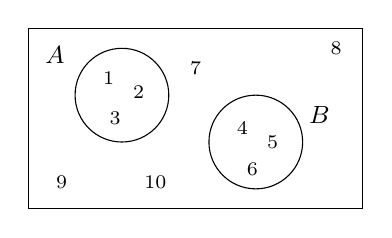
\begin{tikzpicture}[scale=0.85,font=\small]
\draw (0,0) rectangle (5,2.7);
\draw (1.4,1.7) circle (0.7); \draw (3.4,1.0) circle (0.7);
\node at (0.4,2.3) {$A$}; \node at (4.35,1.4) {$B$};
\node at (1.2,1.95) {\scriptsize1}; \node at (1.65,1.75) {\scriptsize2}; \node at (1.3,1.35) {\scriptsize3};
\node at (3.2,1.2) {\scriptsize4}; \node at (3.65,1.0) {\scriptsize5}; \node at (3.35,0.6) {\scriptsize6};
\node at (2.5,2.1) {\scriptsize7}; \node at (4.6,2.4) {\scriptsize8}; \node at (0.5,0.4) {\scriptsize9}; \node at (1.9,0.4) {\scriptsize10};
\end{tikzpicture}}
\Opts{$32$}{$64$}{$128$}{$256$}}
\QQ{33}{\Moslash{Rasmda qirralari $15$ cm, $15$ cm va $1$ m bölgan töğri parallelepipeddan qirqib olingan karniz tasvirlangan. Qirqilgan qismning köndalang kesimi çegarasi $3$ cm li kesma va radiuslari $4$ cm, $5$ cm bölgan ikkita çorak aylanadan iborat ($\pi\approx3$ deb oling).
\par\centering\begin{tikzpicture}[scale=0.19,font=\scriptsize]
\coordinate (d) at (20,10);
\draw (0,15)--(15,15)--(15,0)--(12,0) arc (0:90:5) arc (-90:-180:4) -- (0,9) -- cycle;
\draw (0,15)--($(0,15)+(d)$)--($(15,15)+(d)$)--($(15,0)+(d)$)--(15,0); \draw (15,15)--($(15,15)+(d)$);
\draw[dashed] (0,9)--($(0,9)+(d)$); \draw[dashed] (12,0)--($(12,0)+(d)$)--($(15,0)+(d)$);
\draw[dashed] (3,9)--(7,9)--(7,0)--(12,0);
\node[left] at (0,12) {$6$ cm}; \node[above] at (1.5,9) {$3$}; \node[right] at (7,7) {$4$ cm}; \node[left] at (7,2.5) {$5$ cm}; \node[below] at (13.5,0) {$3$ cm};
\node[above] at (7.5,15) {$15$ cm}; \node[below right] at (25,5) {$1$ m};
\end{tikzpicture}}{A) $155{,}25$\par B) $15525$\par C) $15825$\par D) $58{,}605$\par E) $56{,}805$\par F) $125625$}{Hosil bölgan jismning köndalang kesim yuzini toping (cm$^2$).}{Töla sirtining yuzini toping (dm$^2$).}{Hajmini toping (cm$^3$).}}
\QQ{36}{$\left(x^2-2x+k\right)^2+3x\left(x^2+2x+k\right)=30x^2$ tenglama berilgan. Tenglama yagona ildizga ega böladigan $k$ ning qiymati $k_1$ bölsin. Tenglama ikkita, uçta va törtta ildizga ega böladigan $k$ ning butun qiymatlarining eng kattalari mos ravişda $k_2$, $k_3$, $k_4$ lar bölsin.
\AB{Tenglama yeçimga ega bölmaydigan $k$ ning eng kiçik butun qiymatini toping.}{$k_1\cdot k_3\cdot(k_2+k_4)$ ning qiymatini toping.}}
\QQ{37}{$\sqrt{6x-5-x^2}\cdot\left(\cos2x-\dfrac12\right)=0$ tenglamani yeçing.
\AB{Tenglama neçta haqiqiy ildizga ega?}{Tenglamaning eng kiçik musbat haqiqiy ildizini toping.}}
\QQ{38}{$ABCD$ töğri törtburçak şaklidagi yerning $A$ nuqtasida suv ombori va $C$ nuqtasida issiqxona tasvirlangan. Suv omboridan issiqxonaga $A$ dan $E$ orqali $C$ nuqtaga suv olib boriş uçun $AE$ yöl böyiça soatiga $3$ m, $EC$ yöl böyiça esa soatiga $5$ m tezlikda ariq qazilmoqda. Bunda $AB=30$ m, $BC=80$ m.
\qfig{\begin{tikzpicture}[scale=0.75,font=\small]
\fill[qfill] (0,0) rectangle (8,3); \draw (0,0) rectangle (8,3);
\draw[line width=2.2pt,black!60] (0,0)--(2.25,3)--(8,3); \draw[line width=1.2pt,white] (0,0)--(2.25,3)--(8,3);
\node at (5,1.5) {Yer maydoni};
\node[below left] at (0,0) {$A$}; \node[above left] at (0,3) {$B$}; \node[above] at (2.25,3) {$E$}; \node[above right] at (8,3) {$C$}; \node[below right] at (8,0) {$D$};
\end{tikzpicture}}
\AB{Agar ariq ötkaziş uçun eng minimal vaqt sarflangan bölsa, suv omboridan issiqxonagaça bölgan ariqni qaziş uçun qança vaqt sarflangan?}{Ariq qaziş minimal vaqtda bajarilgan bölsa, $EC$ ariq uzunligini toping.}}
\QQ{39}{$ABCD$ rombning $AB$ tomoniga $DH$ balandlik tuşirilgan, $AH:HB=3:2$ nisbatda böladi. Rombga $DC$ tomoniga $M$ nuqtada urinuvçi doira içki çizilgan.
\qfig{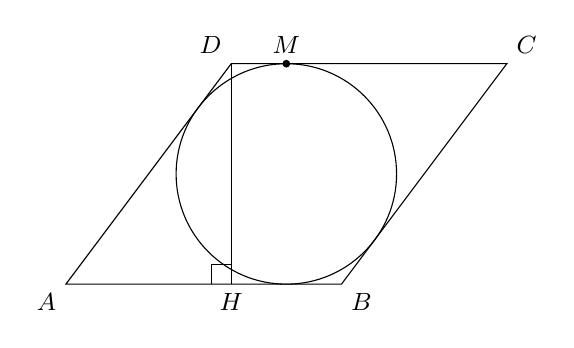
\begin{tikzpicture}[scale=0.7,font=\small]
\coordinate (A) at (0,0); \coordinate (B) at (5,0); \coordinate (C) at (8,4); \coordinate (D) at (3,4); \coordinate (H) at (3,0); \coordinate (M) at (4,4);
\draw (A)--(B)--(C)--(D)--cycle; \draw (D)--(H); \draw (4,2) circle (2); \fill (M) circle (2pt);
\draw (3,0.35)--(2.65,0.35)--(2.65,0);
\node[below left] at (A) {$A$}; \node[below right] at (B) {$B$}; \node[above right] at (C) {$C$}; \node[above left] at (D) {$D$}; \node[below] at (H) {$H$}; \node[above] at (M) {$M$};
\end{tikzpicture}}
\AB{Romb yuzining doira yuziga nisbatini toping ($\pi\approx3$ deb oling).}{$|CM|:|MD|$ nisbatini toping.}}
\QQ{40}{Silindrga muntazam oltiburçakli piramida içki çizilgan. Piramida uçi silindr yuqori asosida, piramida asosi silindr asosida joylaşgan. Silindr va piramida yon sirtlarining nisbati $\dfrac{\sqrt2\pi}3$ ga teng.
\qfig{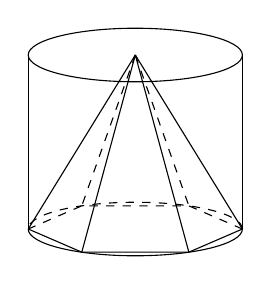
\begin{tikzpicture}[scale=0.85,font=\small]
\draw (-1.6,0)--(-1.6,2.6); \draw (1.6,0)--(1.6,2.6); \draw (0,2.6) ellipse (1.6 and 0.4);
\draw (-1.6,0) arc (180:360:1.6 and 0.4); \draw[dashed] (1.6,0) arc (0:180:1.6 and 0.4);
\coordinate (S) at (0,2.6);
\coordinate (P1) at (1.6,0); \coordinate (P2) at (0.8,0.346); \coordinate (P3) at (-0.8,0.346); \coordinate (P4) at (-1.6,0); \coordinate (P5) at (-0.8,-0.346); \coordinate (P6) at (0.8,-0.346);
\draw (P4)--(P5)--(P6)--(P1); \draw[dashed] (P1)--(P2)--(P3)--(P4);
\draw (S)--(P4); \draw (S)--(P5); \draw (S)--(P6); \draw (S)--(P1); \draw[dashed] (S)--(P2); \draw[dashed] (S)--(P3);
\end{tikzpicture}}
\AB{Silindr va piramida hajmlarining nisbatini toping.}{Piramida apofemasi asos tekisligi bilan qanday burçak taşkil qiladi?}}
\QQ{41}{$f(x)+4f\left(\dfrac1x\right)=\dfrac1x$ funksional tenglama berilgan.
\AB{$f\left(\dfrac12\right)$ ning qiymatini toping.}{$f(x)$ funksiya grafigiga $x_0=1$ nuqtada ötkazilgan urinmaning burçak koeffitsiyentini toping.}}
\QQ{42}{Töğri burçakli uçburçakda $CM$ mediana va $BL$ bissektrisa. Bunda $BL=\dfrac8{\sqrt3}$, $BC=8$ ga teng.
\qfig{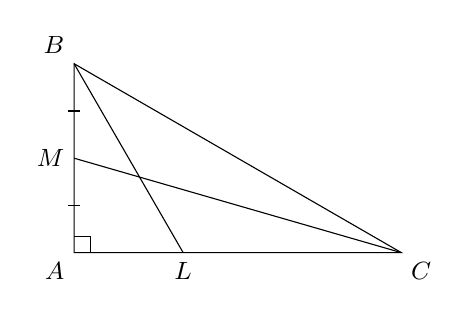
\begin{tikzpicture}[scale=0.6,font=\small]
\coordinate (A) at (0,0); \coordinate (B) at (0,4); \coordinate (C) at (6.928,0); \coordinate (M) at (0,2); \coordinate (L) at (2.309,0);
\draw (A)--(B)--(C)--cycle; \draw (B)--(L); \draw (C)--(M); \draw (0,0.35)--(0.35,0.35)--(0.35,0);
\draw (-0.12,1)--(0.12,1); \draw (-0.12,3)--(0.12,3);
\node[below left] at (A) {$A$}; \node[above left] at (B) {$B$}; \node[below right] at (C) {$C$}; \node[left] at (M) {$M$}; \node[below] at (L) {$L$};
\end{tikzpicture}}
\AB{Kiçik katet uzunligini toping.}{$CM$ mediana uzunligini toping.}}
\QQ{43}{Muntazam sakkizburçakka aylana, aylanaga muntazam oltiburçak içki çizilgan. Sakkizburçak tomoni $a$ ga, oltiburçak tomoni $b$ ga teng.
\qfig{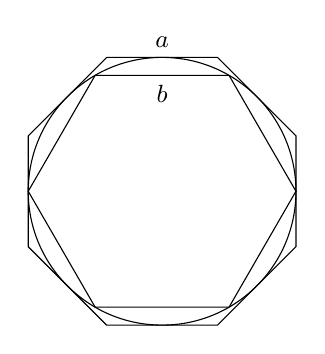
\begin{tikzpicture}[scale=0.85,font=\small]
\draw (22.5:2.165)--(67.5:2.165)--(112.5:2.165)--(157.5:2.165)--(202.5:2.165)--(247.5:2.165)--(292.5:2.165)--(337.5:2.165)--cycle;
\draw (0,0) circle (2);
\draw (0:2)--(60:2)--(120:2)--(180:2)--(240:2)--(300:2)--cycle;
\node[above] at (0,2) {$a$}; \node[below] at (0,1.732) {$b$};
\end{tikzpicture}}
\AB{$\dfrac ab$ nisbatni toping.}{Muntazam oltiburçak yuzi $3\sqrt6+3\sqrt3$ ga teng bölsa, sakkizburçak yuzini toping.}}
\QQ{44}{$f(x)=\sqrt{4-x^2}+2$ funksiya berilgan.
\AB{Koordinatalar boşidan funksiya grafigigaça bölgan eng qisqa masofani toping.}{$\displaystyle\int_0^2f(x)\,dx$ integralni hisoblang.}}
\QQ{45}{$ABC$ uçburçak şaklidagi konsert maydonini quriş uçun $ABC$ uçburçak şaklidagi qismiga beton quyildi va uning parabola şaklidagi qismi taxta bilan qoplandi. $AC$ va $BC$ tomonlar parabolaga urinadi.
\qfig{\begin{tikzpicture}[scale=0.55,font=\small]
\coordinate (A) at (0,0); \coordinate (B) at (10,0); \coordinate (C) at (5,4.444);
\fill[qfill] plot[domain=2:8,samples=40] (\x,{4-4/9*(\x-5)^2}) -- cycle;
\draw (A)--(B)--(C)--cycle; \draw[thick,domain=2:8,samples=40] plot (\x,{4-4/9*(\x-5)^2}); \draw[dashed] (5,0)--(5,4);
\node[below left] at (A) {$A$}; \node[below right] at (B) {$B$}; \node[above] at (C) {$C$};
\node[below] at (1,0) {$2$}; \node[below] at (3.5,0) {$3$}; \node[below] at (6.5,0) {$3$}; \node[below] at (9,0) {$2$}; \node[right] at (5,2) {$4$};
\end{tikzpicture}}
\AB{Qança yuzadagi taxta işlatilgan?}{Beton bilan qoplangan $ABC$ uçburçak şaklidagi sahnaning yuzini toping.}}
\Javoblar{A D C A C A B C A B B C C B A D A C D D D A A B C C B D C D B C A D B}{%
\OK{36}{$7$}{$225$}\OK{37}{$4$}{$1$}\OK{38}{$24$}{$57{,}5$}\OK{39}{$\dfrac53$}{$4$}\OK{40}{$\dfrac{2\pi}{\sqrt3}$}{$45^\circ$}%
\OK{41}{$0$}{$\dfrac13$}\OK{42}{$4$}{$2\sqrt{13}$}\OK{43}{$2\sqrt2-2$}{$16$}\OK{44}{$2\sqrt2$}{$\pi+4$}\OK{45}{$16$}{$22\dfrac29$}}
